\documentclass[
		11pt,
		a4paper,
		toc=listof, %% Abbildungs- und Tabellenverzeichnis mit ins Inhaltsverzeichnis
		bibliography=totoc %% Quellenverzeichnis mit ins Inhaltsverzeichnis
		]{scrreprt}	 %% KOMA Script

% HTWG
\usepackage{graphicx}
\usepackage{a4}
\usepackage{german}

% Eigene
\usepackage[utf8]{inputenc} %% Umlaute
\usepackage[dua]{acronym} %% Abkuerzungsverzeichnis (nur verwendete)
\usepackage{todonotes} %% TODOs moeglich mit \todo{}
\usepackage{booktabs} %% Tabellen
\usepackage{amsmath} %% Formeln
\usepackage{listings} %% Codebeispiele
\usepackage{subfigure} %% Mehrere Bilder nebeneinander
\PassOptionsToPackage{hyphens}{url}\usepackage{hyperref} %% referenzen innerhalb und außerhalb des Dokumentes
\usepackage[headsepline]{scrpage2} %%Numerrierung der Seiten + Kapitelnamen in Kopfzeile inkl. Trennstrich
\pagestyle{scrheadings} %% die folgenden Zeilen sorgen für die korrekte Nummerierung und deren Anzeige 
\clearscrheadfoot %% und für die Kopfzeile mit aktuellem Kapitel etc.
\ihead{\headmark}
\cfoot[\pagemark]{\pagemark}
\automark{chapter}
\usepackage{float} %% Floatpackage um Grafik-Positionen zu forcieren
\newcommand*{\quelle}[1]{\footnotesize Quelle:~#1}

% Eigenes Design 
%TODO loeschen wenn default HTWG Design (was es nicht wirklich gibt) gewuuenscht ist
\usepackage[bottom=3cm]{geometry}
\usepackage{setspace}
\onehalfspacing


% KOMA script anpassungen 
%TODO entfernen wenn kein KOMA Script gewuenscht
\usepackage{scrhack}

%%%%%%%% Codebeispiele
\usepackage{color}
\usepackage{xcolor}
\usepackage{listings}
\usepackage{caption}

\setcounter{tocdepth}{2}  %% Uebreschriften bis subsectionw ins Inhaltsverzeichnis
\setcounter{secnumdepth}{3}  %% Nummerierung bis subsection


%%% Codebeispiele - Style
\DeclareCaptionFont{white}{\color{white}}
\DeclareCaptionFormat{listing}{\colorbox{gray}{\parbox{\textwidth}{#1#2#3}}}
\captionsetup[lstlisting]{format=listing,labelfont=white,textfont=white}

% Entfernt Kapitel Ueberschrift
% Bsp.
% 	ALT:
%       Kapitel 1
%       Einführung
%
% 	NEU:
% 		1 Einführung
%
\renewcommand*\chapterheadstartvskip{\vspace{-\topskip}}
\newcommand{\thema}{Dokumentation Teamprojekt}
\newcommand{\forschungsfrage}{Autonomes Fahren in der DuckieTown-Umgebung - Lokalisierung mit einem Deep-Learning Ansatz}
\newcommand{\abgabedatum}{\today}
\newcommand{\firstauthor}{Stephan Perren}
\newcommand{\secondauthor}{Felix Mayer}
\newcommand{\studiengang}{Angewandte Informatik}
\newcommand{\betreuer}{Prof. Dr. Oliver Bittel}



\begin{document}
%% Nummerierung aus
\pagenumbering{gobble}

% HTWG Templates fuer Titelseite etc.

\begin{titlepage}

\vspace*{-3.5cm}

\begin{center}

\includegraphics[width=5cm]{htwg/htwg-logo}

Fakultät Informatik \\
Fachbereich Wirtschaftsinformatik
\end{center}

\vspace*{1.5cm}

\begin{center}
	\huge{
		\textbf{\thema} \\[1cm]
	}
	\normalsize{
		\textbf{\forschungsfrage} \\[2cm]
	}
\end{center}
\begin{tabular}{p{6cm}p{5cm}}
                 \bfseries{Name:} & \autor \\\\
                 \bfseries{Arbeitsplatz:} & \firma  \\\\
                 \bfseries{Erstkorrektor:} & \erstbetreuer \\\\
                 \bfseries{Zweitkorrektor:} & \zweitbetreuer \\\\
                 \bfseries{Abgabetermin:} & \abgabedatum \\\\
\end{tabular}
\\[1cm]
\begin{flushright}
	Konstanz, \abgabedatum \\[0.5cm]
	Der Vorsitzende des Prüfungsausschusses \\[1.5cm]
	Prof. Dr. Wilhelm Erben
\end{flushright}
\end{titlepage}
\pagenumbering{Roman}
\tableofcontents
\addcontentsline{toc}{chapter}{Inhaltsverzeichnis}
\addchap{Abkürzungsverzeichnis}

\begin{acronym}[ROS]
	\acro{mit}[MIT]{Massachusetts Institute of Technology}
	\acro{ain}[AIN]{Angewandte Informatik}
	\acro{ros}[ROS]{Robot Operating System}
\end{acronym}


\clearpage
%% Starte Paginierung
\pagenumbering{arabic}

\chapter{Einleitung}

\begin{figure}[H]
	\centering
	\begin{minipage}{.5\textwidth}
		\centering
		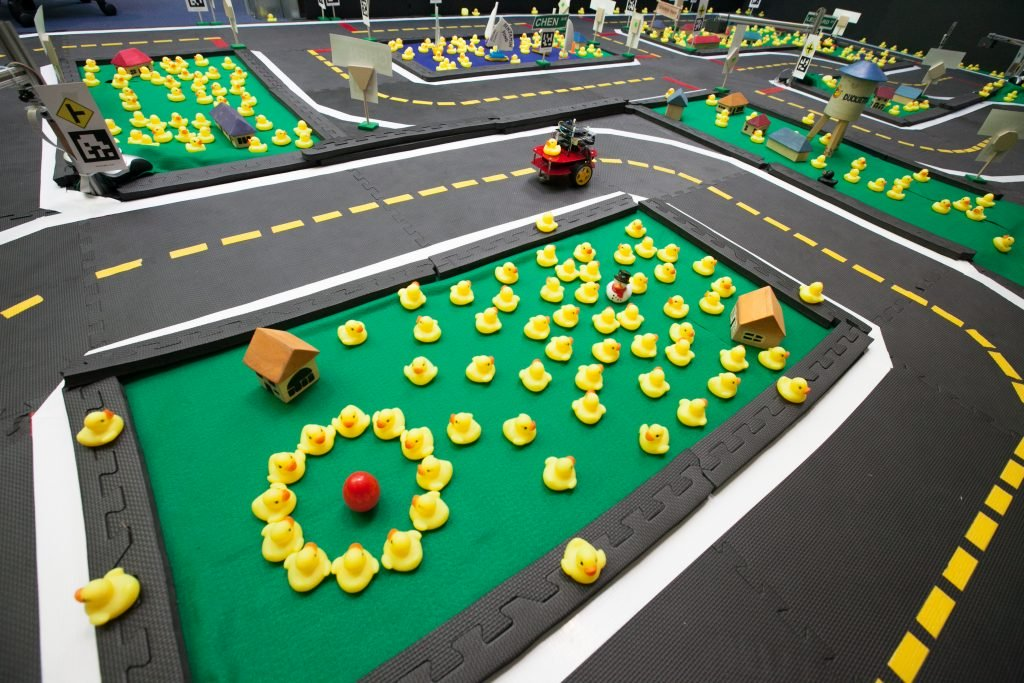
\includegraphics[width=0.95\textwidth]{kapitel1/images/duckietown.png}
		\quelle\url{https://www.duckietown.org/wp-content/uploads/2018/05/duckietown_nice-1024x683.jpg}
		\label{fig:duckietown}
	\end{minipage}%
	\begin{minipage}{.5\textwidth}
		\centering
		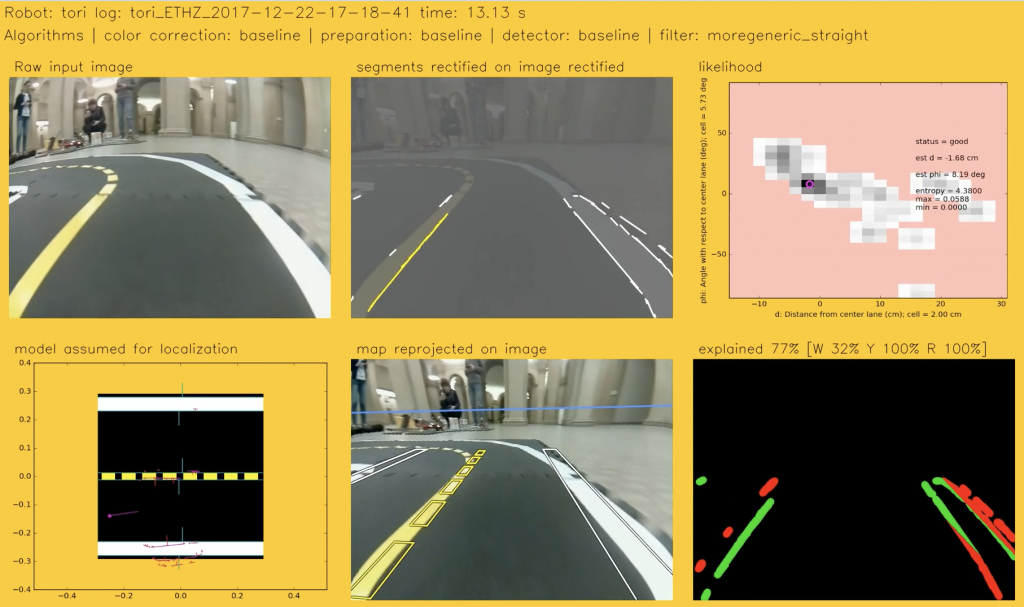
\includegraphics[width=1.072\textwidth]{kapitel1/images/duckietown2.png}
		\quelle\url{https://www.duckietown.org/wp-content/uploads/2018/06/data-from-img-CameraDataProcessed-fc6fd822-1024x607.png}
		\label{fig:duckietown2}
	\end{minipage}
	\caption{Duckietown}
\end{figure}

Das Duckietown-Projekt wurde 2016 am \acf{mit} konzipiert. Das Ziel war es, eine Plattform zu
entwickeln, die klein, kostengünstig und \grqq smart\grqq{} ist, aber dennoch die wissenschaftlichen
Herausforderungen einer echten autonomen Roboterplattform anbietet und die Entwicklung
intelligenter autonomer Fahrfunktionen erlaubt. \cite{duckietown}\\

\noindent Ziel des AIN-Projekts ist die Implementierung verschiedener klassischer Robotik-Algorithmen
für Navigation und Lokalisierung mit dem Duckietown-Simulator\\

\noindent Nach einer Einarbeitung in die Fähigkeiten des Simulators sollen Algorithmen für die
Linienverfolgung, Lokalisierung mit einem Partikelfilter bei bekannter Umgebungskarte,
Navigation (Planung, Wegeverfolgung und Hindernisvermeidung) realisiert werden. Ein Multi-
Vehicle-Szenario soll berücksichtigt werden. Optional können auch KI-Komponenten für
Fahrverhalten und Erkennung von Verkehrszeichen entwickelt werden. Hierzu sollen neue
Techniken wie Deep Neural Networks und Deep Reinforcement Learning zum Einsatz
kommen.\\

\noindent Das Projekt, das für etwa 2-4 Personen vorgesehen ist, soll in Python realisiert werden.
Eventuell kommt \acf{ros} zum Einsatz.

\chapter{Grundlagen}
\section{Abschnitt} 
\subsection{Unterabschnitt}
\begin{figure}
\makebox[\textwidth]{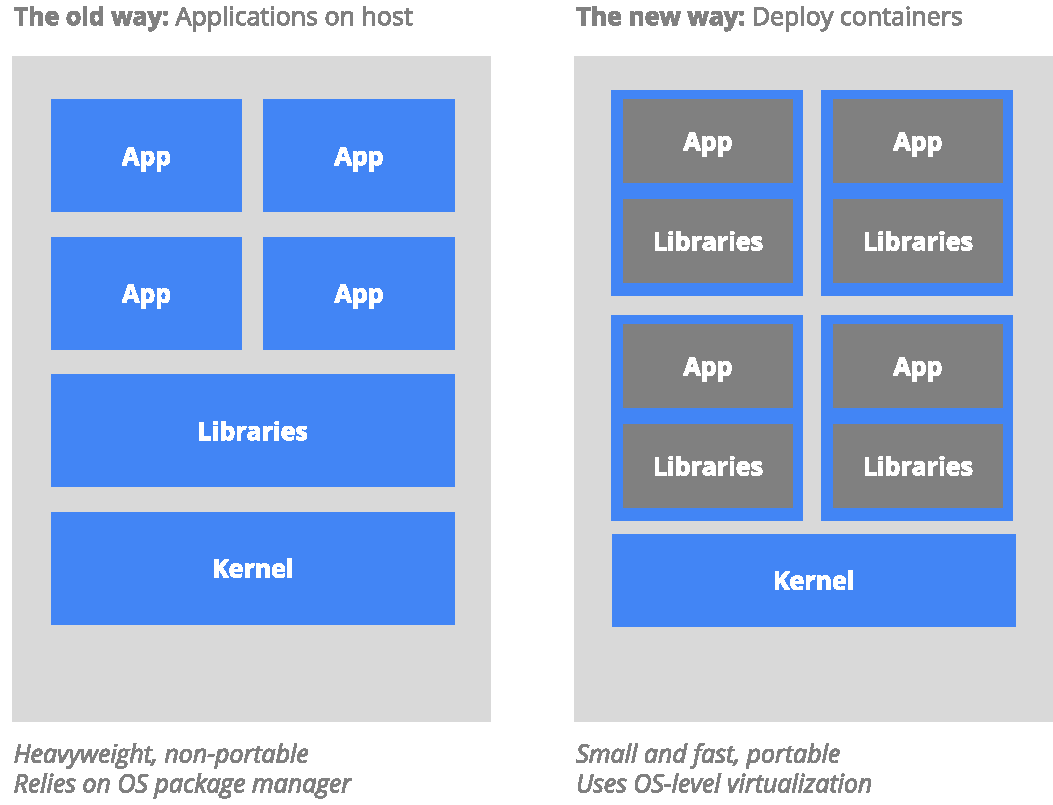
\includegraphics[width=\linewidth]{kapitel2/images/Platzhalter}}
\caption{Bildunterschrift}
\quelle\url{https://tinyurl.com/k3q2n7u} 
\label{Grundlagen:LabelDesPlatzhalters}
\end{figure}

Hier ist ein beispielhafter Verweis auf das Bild: \ref{Grundlagen:LabelDesPlatzhalters} 
Hierfür zitieren wir noch \cite{Anderson.2015}

\chapter{Konzept}



\chapter{Implementierung}


\chapter{Evaluation}


\chapter{Fazit und Ausblick}

\listoffigures
\bibliographystyle{unsrt}
\bibliography{citeulike} 
\end{document}

